\section{ELMo} \label{sec:ELMo}


\subsection{Combing Back To Polysemy} \label{sec:PolysemyAgainInElmo} 

As previously explained, \textbf{\hyperref[sec:Polysemy]{polysemy}} refers to a word's distinct meanings. \hyperref[sec:SolutionWithContextEmbs]{Contextual embeddings} outperform traditional embeddings on \hyperref[app:Appendix_NLPTasks]{nlp tasks} since they assign distinct word vectors per token given a context, as opposed to collapsing all senses within one vector (Wiedemann et al., 2019). Otherwise, homonyms like ``book" (text) and ``book" (reservation) would be assigned the same vector representation even though these are different words.


\subsection{Motivation for ELMo} 

\textbf{ELMo (Embeddings from Language Models)} are ``learned functions of the internal states of a \hyperref[sec:BidirectionalLM]{bidirectional language model (biLM)}" that is pretrained on a large corpus. ELMo representations are \emph{deep} since they are derived from all the \hyperref[sec:BidirectionalLM]{biLM}'s internal layers. 
%ELMo learns a ``linear combination of vectors stacked above each input word for each end task," improving performance of models that use only the top \hyperref[sec:LSTM]{LSTM} layer.  

Higher-level LSTM layers in the ELMo model capture contextual meaning, useful for supervised \nameref{nlptask:wordsensedisambiguatioNWSD}, and lower layers capture syntax information, useful for \nameref{nlptask:postagging}. Mixing these signals allows the learned embeddings select the types of semi-supervision most needed for each end task, so ELMo embeddings end up richer than traditional embeddings (Peters et al., 2018). 


\subsection{Describing ELMo} 

``ELMo is a task-specific combination of the intermediate layer representations in the \hyperref[sec:BidirectionalLM]{biLM}" (Peters et al., 2018). In \cref{eq:ElmoRvector}, for each word token $t_k$, an $L$-layer \hyperref[sec:BidirectionalLM]{biLM} creates $2L + 1$ representations: 

\begin{equation}
\begin{array}{ll}
R_k 
&= \Big \{ \mathbf{x}_k^{LM}, \; \overrightarrow{\mathbf{h}}_{kj}^{LM}, \; \overleftarrow{\mathbf{h}}_{kj}^{LM} \; | \; j = 1,...,L \Big \} \\
&= \Big \{ \mathbf{h}_{kj}^{LM} \; | \; j = 1,...,L \Big \}
\end{array}
\label{eq:ElmoRvector}
\end{equation}

where $\mathbf{h}_{k0}^{LM}$ is the token layer and the hidden state vector $\mathbf{h}_{kj}^{LM} = \Big \{ \overrightarrow{\mathbf{h}}_{kj}^{LM}, \; \overleftarrow{\mathbf{h}}_{kj}^{LM}  \}$, a concatenation of backward and forward hidden states, for each \hyperref[sec:BidirectionalLM]{bidirectional} \hyperref[sec:LSTM]{LSTM} layer. ELMo model collapses all layers in the above vector into a single ELMo embedding ready for a specific task, by weighting the \hyperref[sec:BidirectionalLM]{biLM} layers in a task-specific way, as shown in \cref{eq:ElmoTaskSpecific}: 

\begin{equation}
\textbf{ELMo}_k^{task} = E \Big( R_k; \theta^{task} \Big) = \gamma^{task} \; \sum_{j=0}^L s_j^{task} \; \mathbf{h}_{kj}^{LM}
\label{eq:ElmoTaskSpecific}
\end{equation}

where the vector $\mathbf{s}^{task} = \Big\{ s_j^{task} \Big\}$ of softmax-normalized weights and task-dependent scalar parameter $\gamma^{task}$ allow the model for the specific $task$ to scale the entire $\textbf{ELMo}_k^{task}$ vector. The index $k$ corresponds to a $k$-th word, and index $j$ corresponds to the $j$-th layer out of $L$ layers. Here, $h_{kj}^{LM}$ is the output of the $j$-th \hyperref[sec:LSTM]{LSTM} for word $k$, and $s_j$ is the weight of $h_{kj}^{LM}$ used to compute the representation for word $k$ (Peters et al., 2018).

ELMo can be applied to specific tasks by concatenating the ELMo word embeddings with \hyperref[sec:StaticVsContextualEmb]{context-free word embeddings}, such as those from \nameref{sec:Glove}, to be fed into a task-specific \hyperref[sec:RNN]{RNN} for processing. 





\subsubsection{ELMo's Key Feature} \label{sec:ELMoKeyFeature}



{

\begin{wrapfigure}{L}{0.75\textwidth}
\begin{center}
    \vspace{-18pt}
    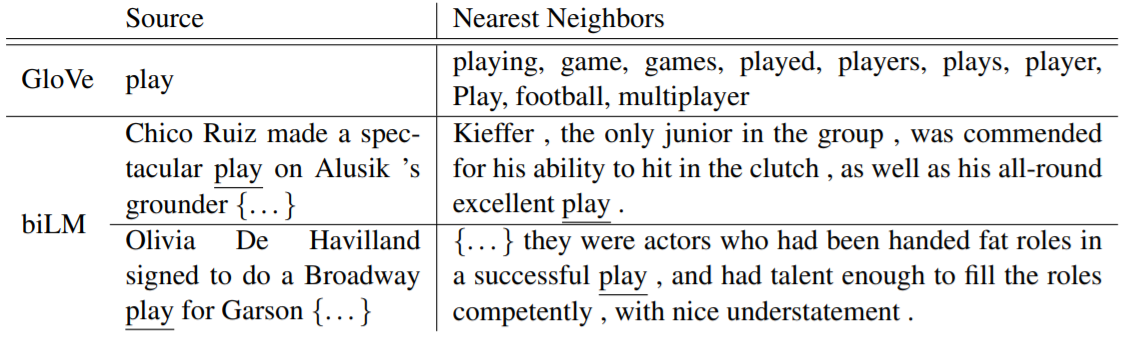
\includegraphics[width=\linewidth]{imgs/table_elmoPlayExamples.png}
\end{center}
\vspace{-15pt}
\captionof{table}{Nearest neighbors to ``play” using GloVe and the context embeddings from a biLM. From Table 4 in \emph{Deep Contextualized Word Representations}, by Peters et al., 2018. \url{https://arxiv.org/pdf/1802.05365.pdf}. Copyright 2018 by Peters et al.}
%\vspace{15pt}
\label{tbl:elmoPlayExample}
\end{wrapfigure}


Peters et al. (2018) found that ELMo's \hyperref[sec:BidirectionalLM]{biLM} contextual vector outputs encode task-specific information that traditional word vectors do not capture. 

To illustrate, consider \cref{tbl:elmoPlayExample}. The word ``play" is highly \hyperref[sec:PolysemyAgainInElmo]{polysemous} since it has many different meanings. To contrast performance of traditional and ELMo embeddings on capturing \hyperref[sec:Polysemy]{polysemy}, Peters et al. (2018) compared words nearest to ``play" found using \nameref{sec:Glove} embeddings with those found using ELMo's \hyperref[sec:BidirectionalLM]{biLM}. 



\nameref{sec:Glove}'s neighbors include several different parts of speech, like verbs (``played", ``playing"), and nouns (``player", ``game") and only in the sport sense of the word. However, the bottom two rows show that the nearest neighbor sentences from the \hyperref[sec:BidirectionalLM]{biLM}'s contextual embedding of ``play" can disambiguate between \emph{both} the parts of speech \emph{and} word sense of ``play". The last row's input sentence contains the noun / acting sense of ``play" and this is matched in the nearest neighbor sentence, highlighting ELMo's ability to learn context using \nameref{nlptask:postagging} and \nameref{nlptask:wordsensedisambiguatioNWSD}. 

}
